% =========================================================
% PART IV -- FREQUENTIST STATISTICS
% =========================================================

\section{Frequentist Statistics}

% ---------------------------------------------------------
% 22. INTRODUCTION TO FREQUENTIST STATISTICS
% ---------------------------------------------------------

\begin{frame}{22. Frequentist Statistics}

\textbf{Definition}

Frequentist statistics is an approach in which unknown population
parameters are studied using data obtained from repeated
sampling.

\vspace{0.4cm}

\textbf{Key ideas}

\begin{itemize}
    \item Parameters are fixed but unknown quantities.
    \item Samples are considered random.
    \item Statistical conclusions are based on observed data.
    \item Sampling distributions are used to study the behavior
    of statistical estimators.
\end{itemize}

\vspace{0.3cm}

\textbf{Example}

A population has an unknown mean $\mu$.
A sample is collected and its mean $\bar{x}$ is used to estimate $\mu$.

\end{frame}


% ---------------------------------------------------------
% 23. SAMPLING
% ---------------------------------------------------------

\begin{frame}{23. Sampling}

\textbf{Definition}

Sampling is the process of selecting a subset of observations
from a population for statistical analysis.

\vspace{0.4cm}

\textbf{Why sampling?}

\begin{itemize}
    \item Studying the entire population may be expensive.
    \item It may be time-consuming or impractical.
    \item A representative sample can provide useful information
    about the population.
\end{itemize}

\vspace{0.3cm}

\textbf{Simple Random Sampling}

Each member of the population has an equal probability
of being selected.

\vspace{0.3cm}

\[
\boxed{
\text{Population}
\longrightarrow
\text{Sample}
\longrightarrow
\text{Statistical Analysis}
}
\]

\end{frame}


% ---------------------------------------------------------
% 23.1 SAMPLING -- EXAMPLE
% ---------------------------------------------------------

\begin{frame}{23.1 Sampling -- Example}

\textbf{Example}

Suppose a university has
\[
N=5000
\]
students and we want to estimate the average number of hours
students spend studying each day. Instead of collecting information from all 5,000 students, we select a random sample of n=200 students.

The sample mean \[
\bar{x}
\] can then be used to estimate the population mean
\[
\mu.
\]
The sample should be selected so that it reasonably represents
the population.

\end{frame}


% ---------------------------------------------------------
% 24. SAMPLING DISTRIBUTION
% ---------------------------------------------------------

\begin{frame}{24. Sampling Distribution}

\textbf{Definition}

A sampling distribution is the probability distribution of a
statistic obtained from all possible samples of a given size
from a population.

\vspace{0.4cm}

For example, the sample mean $\bar{X}$ has its own sampling
distribution.

\vspace{0.3cm}

\[
\boxed{
\text{Population}
\rightarrow
\text{Repeated Samples}
\rightarrow
\text{Statistic}
\rightarrow
\text{Sampling Distribution}
}
\]

\vspace{0.3cm}

\textbf{Important}

A sampling distribution describes the \textbf{variability of a
statistic across repeated samples}, not the distribution of the
individual observations.

\end{frame}

% ---------------------------------------------------------
% 24.1 SAMPLING DISTRIBUTION -- FIGURE
% ---------------------------------------------------------

\begin{frame}{24.1 Sampling Distribution -- Figure}

\begin{columns}[T]

\begin{column}{0.56\textwidth}

\centering
\includegraphics[width=\textwidth]{figures/sampling_distribution.png}

\end{column}

\begin{column}{0.45\textwidth}

The bell curve is centered at the population mean 
$\mu$.

\vspace{0.1cm}

Data are distributed into standard-error ranges around the mean.

\vspace{0.1cm}

About 68$\%$ of observations fall within ±1 standard error.

\vspace{0.1cm}

About 95$\%$ fall within ±2 standard errors.

\vspace{0.1cm}

About 99.7$\%$ fall within ±3 standard errors.

\vspace{0.1cm}

The shaded sections represent the percentage of observations in each range.

\end{column}

\end{columns}

\end{frame}

% ---------------------------------------------------------
% 24.2 SAMPLING DISTRIBUTION -- SAMPLE MEAN
% ---------------------------------------------------------

\begin{frame}{24.2 Sampling Distribution -- Sample Mean}

Suppose the population has mean $\mu$ and variance $\sigma^2$. For random samples of size $n$, the sample mean is
\[
\bar{X}
=
\frac{1}{n}
\sum_{i=1}^{n}X_i
\]
Its sampling distribution has:
\[
\boxed{
E[\bar{X}]=\mu
}
\]
\[
\boxed{
\operatorname{Var}(\bar{X})
=
\frac{\sigma^2}{n}
}
\]
Therefore,
\[
\boxed{
\operatorname{SD}(\bar{X})
=
\frac{\sigma}{\sqrt{n}}
}
\]
This quantity is called the \textbf{standard error} of the
sample mean.

\end{frame}


% ---------------------------------------------------------
% 25. STANDARD ERROR
% ---------------------------------------------------------

\begin{frame}{25. Standard Error}

\textbf{Definition}

Standard error (SE) measures the variability of a statistical
estimator across repeated samples.

For the sample mean:
\[
\boxed{
SE(\bar{X})
=
\frac{\sigma}{\sqrt{n}}
}
\]

When the population standard deviation $\sigma$ is unknown,
it is commonly estimated using the sample standard deviation $s$:
\[
\boxed{
SE(\bar{X})
=
\frac{s}{\sqrt{n}}
}
\]

\vspace{0.1cm}

\textbf{Key idea}

As the sample size increases, the standard error of the sample
mean decreases.

\end{frame}


% ---------------------------------------------------------
% 25.1 STANDARD ERROR -- EXAMPLE
% ---------------------------------------------------------

\begin{frame}{25.1 Standard Error -- Example}

\textbf{Example}

Suppose a sample has:
\[
s=10,
\qquad
n=100
\]

The standard error of the sample mean is
\[
SE(\bar{X})
=
\frac{s}{\sqrt{n}}
\]

\[
=
\frac{10}{\sqrt{100}}
=
\frac{10}{10}
\]

\[
\boxed{
SE(\bar{X})=1
}
\]

\textbf{Interpretation}

A larger sample size generally produces a smaller standard error,
making the sample mean a more precise estimator of the population mean.

\end{frame}


% ---------------------------------------------------------
% 26. ESTIMATOR, ESTIMATE AND PARAMETER
% ---------------------------------------------------------

\begin{frame}{26. Estimator, Estimate and Parameter}

\textbf{Parameter}

A parameter is a fixed but unknown numerical characteristic
of a population.
\[
\mu,\quad \sigma^2,\quad p
\]

\vspace{0.1cm}

\textbf{Estimator}

An estimator is a rule or statistic calculated from sample data
that is used to estimate a population parameter.
\[
\hat{\theta}
\]

\vspace{0.1cm}

\textbf{Estimate}

An estimate is the numerical value obtained after applying
the estimator to a particular sample.

\vspace{0.1cm}
\[
\boxed{
\text{Sample Data}
\longrightarrow
\text{Estimator}
\longrightarrow
\text{Parameter}
}
\]

\end{frame}


% ---------------------------------------------------------
% 26.1 ESTIMATOR, ESTIMATE AND PARAMETER -- EXAMPLE
% ---------------------------------------------------------

\begin{frame}{26.1 Estimator, Estimate and Parameter -- Example}

Suppose $\mu$ is the unknown population mean.

The sample mean
\[
\bar{X}
=
\frac{1}{n}
\sum_{i=1}^{n}X_i
\]

is an \textbf{estimator} of $\mu$.

For a particular sample:
\[
X=\{10,20,30,40,50\}
\]
we obtain
\[
\bar{x}=30.
\]

Therefore:

\begin{itemize}
    \item $\mu$ = population parameter
    \item $\bar{X}$ = estimator
    \item $30$ = estimate
\end{itemize}

\end{frame}


% ---------------------------------------------------------
% 27. BIAS AND VARIANCE
% ---------------------------------------------------------

\begin{frame}{27. Bias and Variance}

\textbf{Bias}

Bias measures the difference between the expected value of
an estimator and the true population parameter.
\[
\boxed{
\operatorname{Bias}(\hat{\theta})
=
E[\hat{\theta}]-\theta
}
\]

An estimator is \textbf{unbiased} if
\[
\boxed{
E[\hat{\theta}]=\theta
}
\]

\textbf{Variance}

Variance measures how much an estimator varies across
different samples.
\[
\boxed{
\operatorname{Var}(\hat{\theta})
=
E[(\hat{\theta}-E[\hat{\theta}])^2]
}
\]

\textbf{Key idea}

Bias describes systematic error, while variance describes
sampling variability.

\end{frame}


% ---------------------------------------------------------
% 27.1 BIAS AND VARIANCE -- TRADE-OFF
% ---------------------------------------------------------

\begin{frame}{27.1 Bias and Variance -- Trade-off}

An estimator may have:

\begin{itemize}
    \item Low bias but high variance.
    \item High bias but low variance.
    \item Both low bias and low variance.
    \item Both high bias and high variance.
\end{itemize}

\vspace{0.4cm}

\textbf{Bias--Variance Trade-off}

In statistical modelling and machine learning, reducing
bias may increase variance and vice versa.

\[
\boxed{
\text{Good estimation}
\approx
\text{Balance between Bias and Variance}
}
\]

\textbf{Application}

The bias--variance trade-off is important when selecting
and evaluating machine learning models.

\end{frame}


% ---------------------------------------------------------
% 28. MEAN SQUARE ERROR
% ---------------------------------------------------------

\begin{frame}{28. Mean Square Error}

\textbf{Definition}

Mean Square Error (MSE) measures the average squared difference
between an estimator and the true parameter.

\vspace{0.4cm}

For an estimator $\hat{\theta}$ of parameter $\theta$:

\[
\boxed{
MSE(\hat{\theta})
=
E[(\hat{\theta}-\theta)^2]
}
\]

\vspace{0.4cm}

MSE can be decomposed into:

\[
\boxed{
MSE(\hat{\theta})
=
\operatorname{Var}(\hat{\theta})
+
\operatorname{Bias}(\hat{\theta})^2
}
\]

\vspace{0.3cm}

\textbf{Key idea}

MSE combines both the variability and systematic error
of an estimator.

\end{frame}


% ---------------------------------------------------------
% 28.1 MEAN SQUARE ERROR -- INTERPRETATION
% ---------------------------------------------------------

\begin{frame}{28.1 Mean Square Error -- Interpretation}

The decomposition

\[
MSE
=
\operatorname{Variance}
+
\operatorname{Bias}^2
\]

shows that estimation error can arise from two sources.

\vspace{0.4cm}

\begin{itemize}
    \item \textbf{Variance:} Estimator changes across different samples.
    \item \textbf{Bias:} Estimator systematically differs from the true parameter.
\end{itemize}

\vspace{0.4cm}

\textbf{Goal}

A good estimator should generally have a small MSE.

\vspace{0.3cm}

\textbf{Application}

MSE is widely used for evaluating statistical estimators
and regression models.

\end{frame}


% ---------------------------------------------------------
% 29. CONSISTENCY
% ---------------------------------------------------------

\begin{frame}{29. Consistency}

\textbf{Definition}

An estimator is consistent if it approaches the true population
parameter as the sample size becomes very large.

For an estimator $\hat{\theta}_n$ of $\theta$:

\[
\boxed{
\hat{\theta}_n
\xrightarrow{P}
\theta
\quad\text{as } n\rightarrow\infty
}
\]

where $\xrightarrow{P}$ denotes convergence in probability.

\textbf{Interpretation}

As more data becomes available, a consistent estimator becomes
increasingly close to the true parameter.

\textbf{Example}

The sample mean $\bar{X}$ is a consistent estimator of the
population mean $\mu$ under standard random-sampling assumptions.

\end{frame}


% ---------------------------------------------------------
% 30. CENTRAL LIMIT THEOREM
% ---------------------------------------------------------

\begin{frame}{30. Central Limit Theorem}

\textbf{Definition}

The Central Limit Theorem (CLT) states that, under suitable
conditions, the sampling distribution of the sample mean
approaches a normal distribution as the sample size becomes large.

\vspace{0.4cm}

If the population has mean $\mu$ and finite variance $\sigma^2$:

\[
\boxed{
\frac{\bar{X}-\mu}
{\sigma/\sqrt{n}}
\xrightarrow{d}
N(0,1)
}
\]

where $\xrightarrow{d}$ denotes convergence in distribution.

\vspace{0.3cm}

\textbf{Key idea}

The original population distribution does not have to be
normal for the CLT to apply, provided suitable conditions hold.

\end{frame}

% ---------------------------------------------------------
% 30.1 CENTRAL LIMIT THEOREM -- FIGURE
% ---------------------------------------------------------

\begin{frame}{30.1 Central Limit Theorem -- Figure}

\begin{columns}[T]

\begin{column}{0.62\textwidth}

\centering
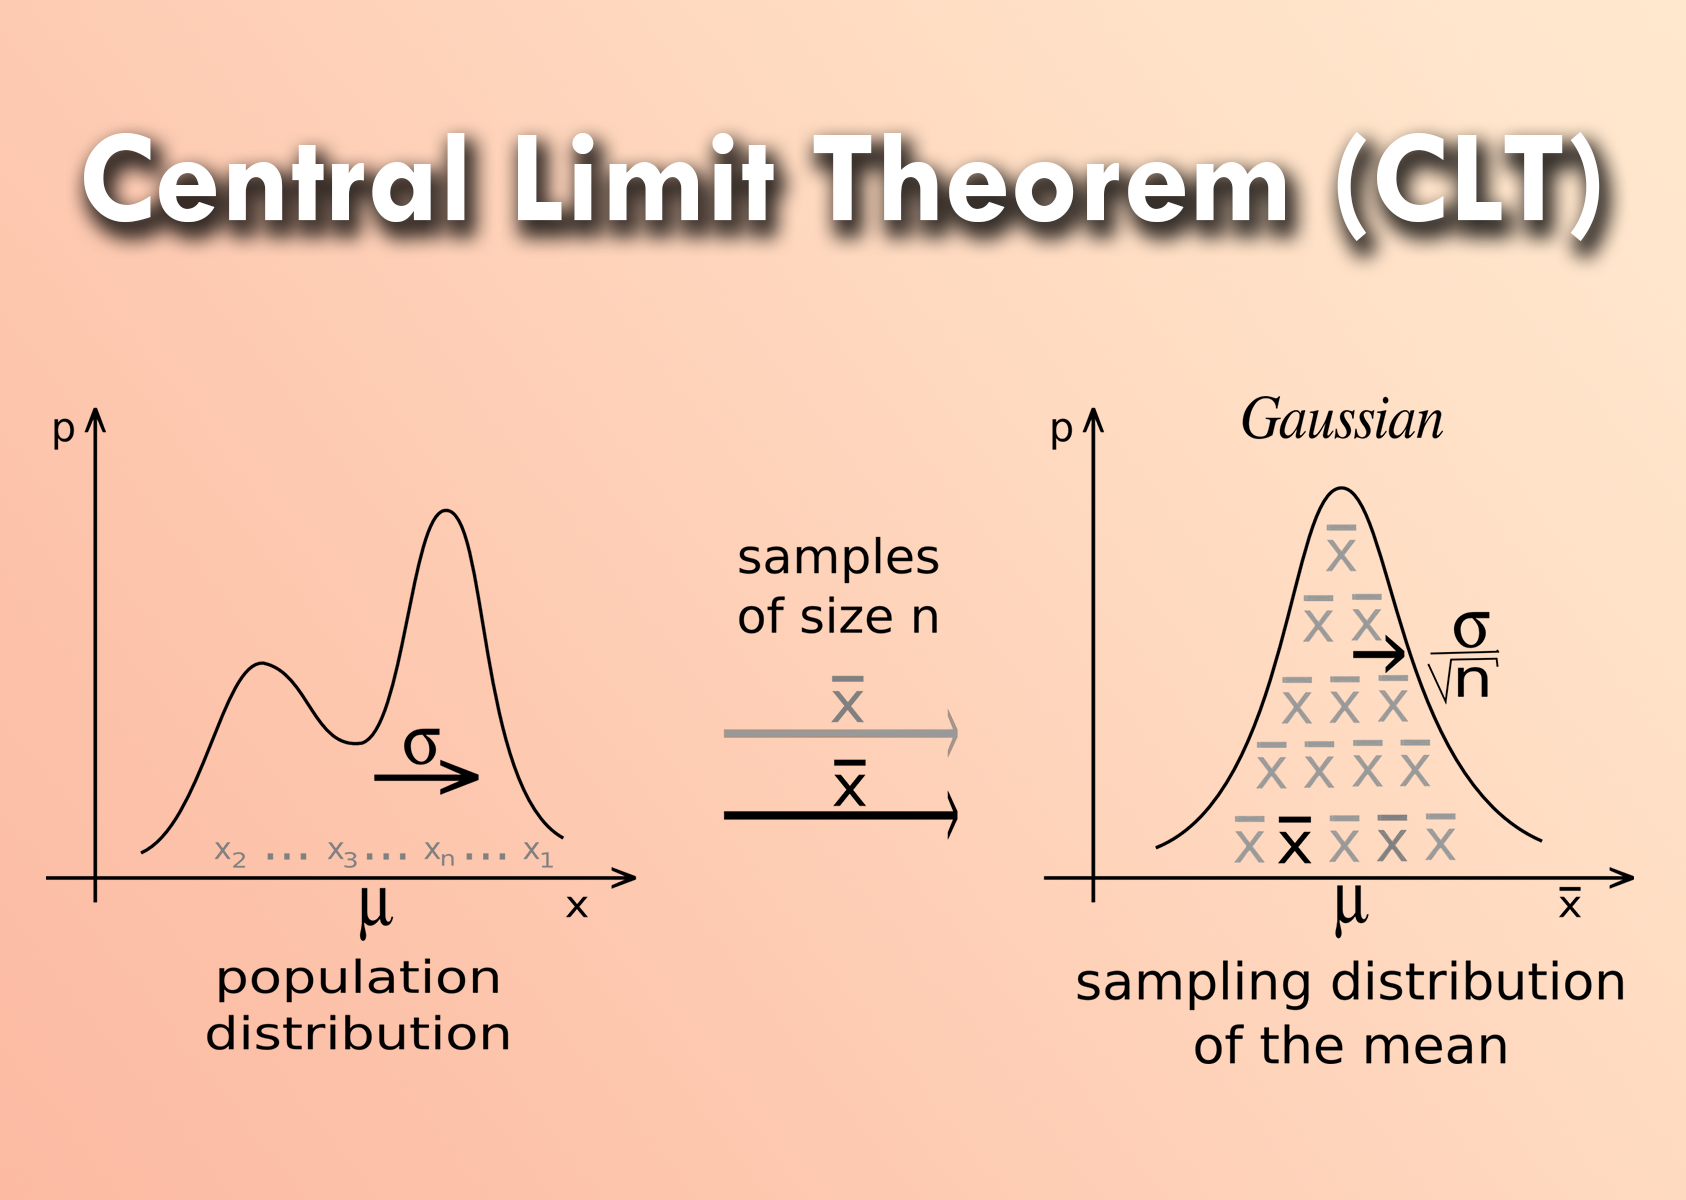
\includegraphics[width=\textwidth]{figures/clt.png}

\end{column}

\begin{column}{0.43\textwidth}

\vspace{0.6cm}

Regardless of the original population’s shape, the distribution of sample means becomes approximately Gaussian (normal) as sample size n increases. 

\vspace{0.4cm}

It is centered at the population mean $\mu$, with standard error $\frac{\sigma}{\sqrt n}$, showing that larger samples produce more precise estimates.

\end{column}

\end{columns}

\end{frame}

% ---------------------------------------------------------
% 30.2 CENTRAL LIMIT THEOREM -- APPLICATION
% ---------------------------------------------------------

\begin{frame}{30.2 Central Limit Theorem -- Application}

\textbf{Why is the CLT important?}

The CLT provides the theoretical basis for many statistical
procedures involving sample means.

\vspace{0.4cm}

It is used in:

\begin{itemize}
    \item Confidence interval construction
    \item Hypothesis testing
    \item Approximation of sampling distributions
    \item Statistical inference from large samples
\end{itemize}

\vspace{0.4cm}

\[
\boxed{
n\uparrow
\quad\Rightarrow\quad
SE(\bar{X})=\frac{\sigma}{\sqrt n}\downarrow
}
\]

\vspace{0.2cm}

Larger samples generally produce more stable estimates of
the population mean.

\end{frame}


% ---------------------------------------------------------
% 31. CONFIDENCE INTERVALS
% ---------------------------------------------------------

\begin{frame}{31. Confidence Intervals}

\textbf{Definition}

A confidence interval is an interval calculated from sample
data that provides a range of plausible values for an unknown
population parameter.

\vspace{0.4cm}

For a population mean with known $\sigma$, a confidence interval
can be written as:

\[
\boxed{
\bar{x}
\pm
z_{\alpha/2}
\frac{\sigma}{\sqrt n}
}
\]

where $z_{\alpha/2}$ is the appropriate standard normal
critical value.

\vspace{0.3cm}

\textbf{General form}

\[
\boxed{
\text{Estimate}
\pm
\text{Margin of Error}
}
\]

\end{frame}


% ---------------------------------------------------------
% 31.1 CONFIDENCE INTERVALS -- EXAMPLE
% ---------------------------------------------------------

\begin{frame}{31.1 Confidence Intervals -- Example}

\textbf{Example}

Suppose:
\[
\bar{x}=50,\qquad
\sigma=10,\qquad
n=100
\]

For a $95\%$ confidence interval:
\[
z_{0.025}=1.96
\]

The margin of error is
\[
1.96\frac{10}{\sqrt{100}}
=
1.96
\]

Therefore,
\[
CI
=
50\pm1.96
\]
\[
\boxed{
CI=(48.04,\;51.96)
}
\]
Using this procedure, the interval obtained from the sample is intended to capture the true population mean in the long-run at the stated confidence level.

\end{frame}


% ---------------------------------------------------------
% 31.2 CONFIDENCE INTERVALS -- KEY POINTS
% ---------------------------------------------------------

\begin{frame}{31.2 Confidence Intervals -- Key Points}

The width of a confidence interval depends on:

\begin{itemize}
    \item Sample size
    \item Variability of the data
    \item Chosen confidence level
\end{itemize}

For the mean:
\[
\boxed{
\text{Margin of Error}
=
z_{\alpha/2}
\frac{\sigma}{\sqrt n}
}
\]

\textbf{Effect of sample size}

\[
n\uparrow
\quad\Rightarrow\quad
\frac{\sigma}{\sqrt n}\downarrow
\]

Therefore, larger samples generally lead to
\textbf{narrower confidence intervals}.

\end{frame}